\chapter{Inner Products}

This chapter covers the following ideas.


\begin{enumerate}

\item Explain the dot product and inner product. Use them to define length and angles of vectors. Normalize vectors, obtain vectors of a given length in a given direction, and explain how to tell if two vectors are orthogonal. 

\item Obtain the orthogonal complement of a set of vectors (relate it to the null space of the transpose). Use the orthogonal complement to project vectors onto vector spaces. 

\item By considering the projection of a vector onto a vector subspace, explain why solving $A^TA \vec x = A^T\vec b$ gives the solution to the least squares regression problem.

\item Use the Gram-Schmidt orthogonalization process to obtain an orthonormal basis of vectors. Show how to compute components of vectors relative to an orthogonal basis (called Fourier coefficients).  

\item Illustrate by examples that when a matrix is symmetric, eigenvectors corresponding to different eigenvalues are orthogonal, which means you can find an orthonormal basis to diagonalize the matrix. 

\end{enumerate}


\section{The Dot Product}

Recall the length of a vector $\vec u = (u_1,u_2)$ in $\R^2$ is (from the Pythagorean theorem) 
$$\norm{\vec u} = |\vec u| = \sqrt{u_1^2+u_2^2}.$$ 
The notation $|\vec u|$ and $\norm{\vec u}$ are both used to denote the length or \textbf{norm} or a vector, 
\marginpar{The norm of a vector is a synonym for the magnitude or length. }
depending on the context and author.  
Repeated use of the Pythagorean theorem gives $$|(u_1,u_2,u_3)|=\sqrt{u_1^2+u_2^2+u_3^2}.$$ 
It seems reasonable to generalize this to $\R^n$ by letting $$|\vec u|=|(u_1,\ldots,u_n)| = \sqrt{u_1^2+\cdots u_n^2}.$$ 
Now that we have spent a semester looking for matrix patterns, notice that the length can be written as a matrix product  $\sqrt{\vec u^T \vec u}$
So the square of the length of a vector is precisely the quantity $$\norm{\vec u}^2 = \vec u^T\vec u.$$  
Mathematicians discovered that sometimes the quantity $\vec u^T\vec v$ appears where $\vec u$ and $\vec v$ are different vectors.  This quantity appeared so often that they gave it a name, the dot product. We'll see some applications in just a bit.
%(The word product is used because when taking the derivative of functions of vectors, the product rule applies to the dot product. Similarly, the matrix product satisfies the product rule, as does any mathematical ``product.'')

\begin{definition}
Given vectors $\vec u = (u_1,u_2,\ldots, u_n)$ and $\vec v = (v_1,v_2,\ldots, v_n)$, define the dot product $\vec u \cdot \vec v$ to be the scalar 
$$\vec u \cdot\vec v = \vec u^T\vec v = u_1v_1+u_2v_2+\cdots u_nv_n = \sum_{i=1}^n u_iv_i. $$
\end{definition}
If $\vec u = \vec v$, then the dot product $\vec u\cdot \vec u= \norm{\vec u}^2$ equals the square of the length of the vector. 
If the length of a vector is 1, we say the vector is a \textbf{unit vector}. 
\marginpar{Unit vectors have length 1.} 
The standard basis vectors for $\R^n$ are unit vectors. 
If a vector is not a unit vector, we can make it a unit vector by dividing by its length. 
Unit vectors give us a way to find vectors of any length in a given direction, all we have to do is multiply a unit vector by the length we want. 
As result, we can write every vector as a product of its norm (length) and a unit vector in the same direction, i.e. we will write $$\vec v= c\vec u\quad \text{where}\quad c=|\vec v|\quad \text{and}\quad\vec u =\frac{\vec v}{|\vec v|} \quad \text{is a unit vector}.$$ 
Much of what we do in this unit will involve decomposing a vectors into the product of its length and direction.


\begin{example}
Let's find a vector of length 7 in the direction of $\vec v = (1,3,-2)$.  

The vector $\vec v = (1,3,-2)$ has length $|\vec v|=\sqrt{1+9+4}=\sqrt{14}$, so a unit vector in the same direction as $(1,3,-2)$ is 
$$\vec u = \frac{\vec v}{|\vec v|}=
\ds\frac{1}{\sqrt{14}}(1,3,-2) 
= \left(\frac{1}{\sqrt{14}},\frac{3}{\sqrt{14}},-\frac{2}{\sqrt{14}}\right).$$
Since the vector $\vec u$ is 1 unit long (its a unit vector), we multiply by 7 to obtain a vector 7 units long in the same direction.  
A vector 7 units long in the same direction as $(1,3,-2)$ is
$$\vec w = 7\vec u = (7)\left(\ds\frac{1}{\sqrt{14}}(1,3,-2)\right) = \left(\frac{7}{\sqrt{14}},\frac{21}{\sqrt{14}},-\frac{14}{\sqrt{14}}\right).$$  
\end{example}

\subsection{Properties of the Dot Product}

Before proceeding to the definition of an inner product, let's pinpoint some properties of the dot product. We'll be using these properties to define inner products on abstract vector spaces. 

\begin{theorem}
The dot product $\vec u \cdot \vec v$ on $\R^n$ satisfies the following properties:
\begin{enumerate}
\item $(\vec u +\vec v)\cdot \vec w = \vec u\cdot \vec w + \vec v\cdot \vec w$ (The dot product preserves vector addition.)
\item $(a\vec u)\cdot \vec v = a(\vec u\cdot \vec v)$ (The dot product preserves scalar multiplication.)
\item $\vec u\cdot \vec v = \vec v\cdot \vec u$ (The dot product is commutative) 
\item $\vec u\cdot \vec u \geq 0$ and $\vec u\cdot\vec u=0$ if and only if $\vec u =\vec 0$ (The dot product is positive definite.)
\end{enumerate}
\end{theorem}

The first two properties imply that the dot product is linear. You can pull out constants and perform the dot product either before or after you multiply.  The third properties shows that it does not matter in which order you perform the dot product. In particular, this implies that the first two properties apply to the right side of the dot product (for example $\vec u \cdot (b\vec v) = b(\vec u \cdot \vec v)$).  The last property just requires that the only way to get out zero when dotting a vector with itself is to use the zero vector. Essentially, we need this property to show that length $|\vec u| =\sqrt{\vec u\cdot \vec u} = 0$ is well defined (as you can't take the square root of negative numbers) and that the only vector whose length is zero is the zero vector itself.

The dot product provides a nice way to compute angles between vectors in $\R^2$ or $\R^3$.  
If $\theta$ is the angle between 2 vectors $\vec u$ and $\vec v$, then we can find the angle between these two vectors using \marginpar{The dot product finds angles: $$\vec u \cdot \vec v = |\vec u||\vec v|\cos \theta$$}
$$\vec u \cdot \vec v = |\vec u||\vec v|\cos \theta.$$
This follows from the law of cosines $c^2 = a^2 + b^2 -2ab \cos \theta$, where $a=|\vec u|$, $b=|\vec v|$, and $c = |\vec u-\vec v|$. 
\marginpar{{%\normalsize
\begin{center}
Law of Cosines
$$c^2=a^2+b^2-2ab\cos\theta$$
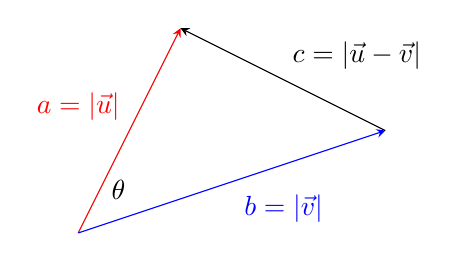
\begin{tikzpicture}[scale=1.3]
%\draw[help lines,step=1cm] (0,0) grid (3,2);
\draw[->,>=stealth,red] (0,0) -- node[above left ,fill=white] {$a=|\vec u|$}(1,2);
\draw[->,>=stealth,blue] (0,0) -- node[below right=1pt,fill=white] {$b=|\vec v|$} (3,1);
%\draw[<-,>=stealth,blue] [shift={(-2,1)}](0,0) -- node[above left=1pt,fill=white]{$-\vec v$} (3,1);
%\draw[->,>=stealth,ultra thick] (0,0) -- node[below left=0pt,fill=white] {$\vec u-\vec v$}(-2,1);
\draw[->,>=stealth,black] [shift={(3,1)}](0,0) -- node[above right=0pt,fill=white] {$c=|\vec u-\vec v|$}(-2,1);
\draw(0,0) node[above right=3mm]{$\theta$};
\end{tikzpicture}
\end{center}
}}
Because the dot product is equal to the square of the magnitude, we have 
$$(\vec u-\vec v)\cdot (\vec u-\vec v) = \vec u\cdot \vec u +\vec v\cdot \vec v -2|\vec u||\vec v|\cos \theta.$$
Distributing on the left gives 
$$\vec u\cdot \vec u - 2 \vec u \cdot \vec v +\vec v\cdot \vec v = \vec u\cdot \vec u +\vec v\cdot \vec v -2|\vec u||\vec v|\cos \theta.$$
Now cancel the common terms on both sides and divide by 2 to obtain our formula $\vec u \cdot \vec v = |\vec u||\vec v|\cos \theta$.  
This formula geometrically explains how to connect the dot product to angles in both 2 and 3 dimensions.  
In higher dimensions we now define the angle between two vectors using this formula.

\begin{definition}[Angle between two vectors]
Let $\vec u$ and $\vec v$ be vectors in $\R^n$. We define the angle $\theta$ between $\vec u$ and $\vec v$ to be the unique angle between 0 and 180 degrees such that 
\marginpar{We can define both lengths and angles entirely in terms of the dot product.}
$$cos \theta 
= \frac{\vec u\cdot \vec v}{|\vec u||\vec v|}
= \frac{\vec u\cdot \vec v}{\sqrt{\vec u\cdot\vec u}\sqrt{\vec v\cdot\vec v}}.$$
\end{definition}
In order to make this generalization, we need to know that $$-1\leq \dfrac{\vec u\cdot\vec v}{|\vec u||\vec v|}\leq 1$$ so that it will always be the cosine of some angle.  
This is equivalent to showing $|\vec u\cdot\vec v|\leq |\vec u||\vec v|$, which is called the Cauchy-Schwartz inequality. A proof of the Cauchy Swartz inequality is on page 275 (problem 7.35) in Schaum's.


When two vectors meet at a 90 degree angle, then $\cos 90^\circ = 0$.  
This means that the dot product is zero since $$\vec u \cdot \vec v = |\vec u||\vec v|\cos 90 = |\vec u||\vec v| 0=0.$$ 
If the dot product is zero, then we know $0=\vec u \cdot \vec v = |\vec u||\vec v|\cos \theta$. Since  $|\vec u||\vec v|\cos \theta=0$, either one of the vectors has zero length or the cosine of the angle between them is zero (hence the angle is 90 degrees). The word perpendicular suggests that two objects meet at a 90 degree angle. If the dot product of two vectors is zero, then they may meet perpendicularly, or one of the vectors might be zero. We create a new word ``orthogonal'' to mean precisely this: the vectors meet at a 90 degree angle or one of the vectors is zero.
\begin{definition}
We say that $\vec u$ and $\vec v$ are orthogonal if their dot product is zero. 
\marginpar{orthogonal = dot product is zero} 
\end{definition}




\begin{example}
The dot product of the two vectors $\vec u = (1,0,3,-4)$ and $\vec v=(3,-1,5,0)$ is $$\vec u\cdot \vec v = (1)(3)+(0)(-2)+(3)(5)+(-4)(0) = 18.$$ 
The length of each vector is $$|\vec u| = \sqrt{9+1+16} = \sqrt{26}\quad\text{and}\quad|\vec v| = \sqrt{9+1+25} = \sqrt{35}.$$ 
The angle between $\vec u$ and $\vec v$ is $$\theta  = \cos ^{-1} \left(\frac{18}{\sqrt{26}\sqrt{35}}\right),$$ which you can obtain in radians or degrees using a calculator.

The dot product of the two vectors $\vec u = (-2,1,3)$ and $\vec v = (1,5,-1)$ is $-2+5-3=0$, so $\cos \theta = 0$ (without finding the lengths). This means that the angle between the vectors is 90 degrees, and the vectors are orthogonal.
\end{example}

When the dot product of two vectors is zero, we say the vectors are orthogonal. Provided neither vector is zero, this means that the angle between the two vectors is 90 degrees.  In summary, dot product helps us
\begin{enumerate}
	\item Find the length of a vector: $\vec u \cdot \vec u=|\vec u |^2$,
	\item Find the angle between two vectors: $\vec u \cdot \vec v = |\vec u||\vec v|\cos \theta$,
	\item Determine if two vectors are orthogonal: $\vec u \cdot \vec v = 0$.
\end{enumerate}
 
 
 
 
 
 
 
 
 
 
 
 
 
\section{The Inner Product - A General Dot product}
In the last section we showed that the dot product is really just the matrix product $$\vec u\cdot \vec v = \vec u^T\vec v.$$ 
This product satisfies the following properties:
\begin{enumerate}
\item $(\vec u +\vec v)\cdot \vec w = \vec u\cdot \vec w + \vec v\cdot \vec w$ (The dot product preserves vector addition.)
\item $(a\vec u)\cdot \vec v = a(\vec u\cdot \vec v)$ (The dot product preserves scalar multiplication.)
\item $\vec u\cdot \vec v = \vec v\cdot \vec u$ (The dot product is commutative) 
\item $\vec u\cdot \vec u \geq 0$ and $\vec u\cdot\vec u=0$ if and only if $\vec u =\vec 0$ (The dot product is positive definite.)
\end{enumerate}
We also use the dot product to obtain lengths using $|\vec u|^2 = \vec u\cdot \vec u$ and angles using $|\vec u||\vec v| \cos\theta = \vec u\dot \vec v$. All of the computations are done in the vector space $\R^n$. We now ask, is there a similar kind of product in other vector spaces, so that we can talk about lengths and angles between abstract vectors in any vector space? This question led to the definition of an inner product.




\begin{definition}
An (real) \textbf{inner product} on a vector space $V$ is a function (written $\left<\vec u,\vec v\right>$) which takes two vectors $\vec u$ and $\vec v$ and returns a numbers $\left<\vec u,\vec v\right>$. This function satisfies the following axioms:
\begin{enumerate}
\item $\left< \vec u +\vec v, \vec w\right> = \left<\vec u, \vec w \right> + \left< \vec v ,    \vec w \right>$ (The inner product preserves vector addition.)
\item $\left< a\vec u ,    \vec v \right>= a\left< \vec u ,    \vec v \right>$ (The inner product preserves scalar multiplication.)
\item $\left< \vec u ,    \vec v  \right> = \left< \vec v ,    \vec u \right>$ (The inner product is commutative) 
\item $\left< \vec u ,    \vec u \right> \geq 0$ and $\left< \vec u ,   \vec u \right>=0$ if and only if $\vec u =\vec 0$ (The inner product is positive definite.)
%	\item $\left<a\vec u +b\vec v,\vec w\right> = a\left<\vec u,\vec w\right> +b\left<\vec v,\vec w\right> $ (it's linear)
%	\item $\left<\vec u,\vec v\right> = \left<\vec v,\vec u\right>$ (it's symmetric) 
% 	\item $\left<\vec u,\vec u\right> \geq 0$ and $\left<\vec u,\vec 0\right> =0$ if and only if $\vec u = \vec 0$. (it's positive definite)
\end{enumerate}
A vector space together with an inner product is called an \textbf{inner product space}.
\end{definition}

The axioms above allow us to treat an inner product in the same way we treat the dot product.  The first two properties imply that the inner product is linear, which basically means we can distribute as in 
$$\left<a\vec u +b\vec v,\vec w\right> = a\left<\vec u,\vec w\right> +b\left<\vec v,\vec w\right>.$$  
If $\left<\vec u,\vec v\right>$ is an inner product on a vector space $V$, then relative to this inner product we can
\begin{enumerate}
	\item 
	\marginpar{When working with an abstract inner product, we normally use double bars $\norm{\vec u}$ instead of single bar $|\vec u|$ to talk about the norm of a vector.}
	Find the norm (length) of a vector: $\left<\vec u , \vec u\right>=\norm{\vec u }^2$,
	\item Find the angle between two vectors :$\left<\vec u , \vec v\right>= \norm{\vec u} \norm{\vec v}\cos \theta$,
	\item Determine if two vectors are orthogonal: $\left<\vec u , \vec v\right> = 0$.
\end{enumerate}
In order to define angles, we need to know that $-1\leq \cos\theta \leq 1$, or $\ds -1\leq \dfrac{\left<\vec u,\vec v\right>}{\norm{\vec u}\ \norm{\vec v}}\leq 1$.  The Cauchy-Swartz inequality (pg 247) verifies that $|\left<\vec u , \vec v\right>|\leq \norm{\vec u} \norm{\vec v}$, which provides the required justification. 
Always remember: the inner product is just a generalization of the dot product which allows us to work with vector spaces  and define lengths and angles just as we did with the dot product. It's time for some examples of inner products.

\begin{example}
The dot product is itself an inner product, as it satisfies the 4 axioms. We will often call the usual inner product on $\R^n$.
\end{example}


\begin{example}
The Federal Communications Commission (FCC) creates regulations about the types of signals that can be broadcast.  
Because of these regulations, signals form a vector space (a vector space of periodic function). In this example, we'll show how to define inner products on a vector space of functions.

Consider the vector space of continuous functions on the interval $[0,1]$. Define an inner product on this space by $\left<f,g\right> = \int_0^1 fg dx$.  If you think of a function as an infinitely long list of numbers, then essentially this inner product requires that you multiply each component $f(x)$ by its corresponding component $g(x)$ and then add up the values from $0$ to $1$ using an integral. It's basically the same as the dot product, just now we have infinitely many values to sum so we use an integral instead of a sum.

We will now show that the inner product $\left<f,g\right> = \int_0^1 fg dx$ is an inner product by showing it satisfies the axioms.
\begin{enumerate}
	\item We need to show that you can add either before or after computing the inner product (we say the inner product distributes across addition or it preserves addition).  
	We compute \begin{align*}
	\left<f +g,h\right> 
	&=\int_0^1(f+g)h\ dx 
	= \int_0^1(fh+gh)\ dx \\
	&= \int_0^1fh\ dx + \int_0^1gh\ dx 
	=  \left<f,h\right> +\left<g,h\right>. 
	\end{align*} 
	Since $\left<f +g,h\right> = \left<f,h\right> +\left<g,h\right>$, this product preserves vector addition.

	\item We need to show that you can multiply by a scalar either before or after computing the inner product (we say the inner product distributes across scalar multiplication or it preserves scalar multiplication).  
	We compute \begin{align*}
	\left<af,g\right> 
	=\int_0^1(af)g\ dx 
	= a\int_0^1fg\ dx 
	=  a\left<f,g\right>.
	\end{align*}
	Since $\left<af,g\right> =a \left<f,g\right>$, this product preserves scalar multiplication.

%	\item $\left<af +bg,h\right> =\int_0^1(af+bg)h\ dx = \int_0^1(afh+bgh)\ dx = a\int_0^1fh\ dx + b\int_0^1gh\ dx =  a\left<f,h\right> +b\left<g,h\right> $ (so it's linear)
	\item We need to show that you can interchange the order of the inner product without changing the value (we say the inner product is commutative). 
	We compute
		 \begin{align*}
		 \left<f,g\right> 
		 =  \int_0^1fg\ dx 
		 = \int_0^1gf\ dx 
		 = \left<g,f\right>
		 \end{align*} 
	Since $\left<f,g\right> =\left<g,f\right>$, this product is commutative. 
 	
 	\item We need to show that the inner product of a nonzero vector with itself always returns a positive number (so that we can use the inner product to define lengths).  We also need to show that the inner product of zero with itself is zero. If both these are satisfied, we say the inner product is positive definite. 
 	We compute $\ds \left<f,f\right> = \int_0^1 f^2 dx$.  Because $f^2 \geq 0$, we know that the area under $f^2$ cannot be negative, so $\int_0^1 f^2dx \geq 0$. If $f\neq 0$ somewhere, then there will be some small interval on which $f$ is positive (because $f$ is continuous). This means $f^2$ will have a nonzero amount of area under it.  Hence $\left<f,f\right> =0$ if and only if $f=0$ 
Because $\left<f,f\right> = \int_0^1 f^2 dx \geq 0$ and equals zero only when $f(x)=0$, this product is positive definite.
\end{enumerate}
We have shown that the inner product $\left<f,g\right> = \int_0^1 fg dx $ is an inner product on the vector space of continuous functions defined on $[0,1]$.  This inner product is closely related to the inner products used by the FCC to establish radio communication.  It is also related to data compression of JPG, MP3, and other electronic formats. 
\end{example}



The previous example showed how to define an inner product on an infinite dimensional vector space.  
Let's now take a look at alternate ways to define inner products on $\R^n$, using symmetric matrices. 
To introduce this example, recall that the dot product is really just the matrix product 
$$\vec u\cdot \vec v = \vec u^T\vec v = \vec u^T I \vec v,$$
where $I$ is the identity matrix inserted between $u^T$ and $v$.
As mathematicians solved various problems, they discovered a pattern that if $A$ is a symmetric matrix (so $A^T=A$) whose eigenvalues are positive, then $\vec u^T A \vec v$ created an inner product. After further work, they then showed that if $\left<\vec u,\vec v\right>$ is an inner product on a finite dimensional vector space, then relative to some basis $S$ you can always find a symmetric matrix $A$ such that 
$$\left<\vec u,\vec v\right> = [\vec u]_S^T A [\vec v]_S$$.  In other words, when dealing with finite dimensional vector spaces, symmetric matrices produce inner products, and inner products produce symmetric matrices. Studying symmetric matrices is the same as studying inner products.

\begin{example}
Let $A$ be a symmetric matrix which satisfies $$\vec x^T A\vec x> 0\quad \text{for}\quad \vec x\neq 0.$$ 
%This condition is equivalent to having real positive eigenvalues, which for now we'll just use it as a fact (we'll see why in a bit). 
Define a new inner product on $\R^n$ by the formula $\left<\vec u,\vec v\right> = \vec u^T A \vec v$. 
Let's show that this provides an inner product on $\R^n$.
\begin{enumerate}
	\item We compute \begin{align*} 
	\left<\vec u +\vec v,\vec w\right> 
	& =(\vec u+\vec v) A \vec w \\
	&=\vec uA\vec w+\vec vA \vec w  \\
	&= \left<\vec u,\vec w\right> +\left<\vec u,\vec w\right> 
	\end{align*}
	which shows it preserves addition.

	\item We compute \begin{align*} 
	\left<a\vec u ,\vec v\right> 
	& =(a\vec u) A \vec v \\
	&=a\vec uA\vec v \\
	&= a\left<\vec u,\vec v\right> 
	\end{align*}
	which shows it preserves scalar multiplication.
	\item Recall that the inner product produces a number, so $\vec u^T A \vec v$ is a number.  
	We compute both 
	$$\left<\vec u ,\vec v\right> = u^TA\vec v 
	\quad\text{and}\quad 
	\left<\vec v ,\vec u\right> = v^TA\vec u
	$$ 
	The transpose of a number is itself, so $\vec u^T A \vec v$ is the same as its transpose $(\vec u^T A \vec v)^T = \vec v^T A^T\vec u$ (remember you reverse the order and transpose each matrix).  
	Since $A$ is symmetric, we can replace $A^T$ with $A$. This means  
	$$\left<\vec u, \vec v \right> = \vec v^T A^T\vec u= \vec v^T A\vec v = \left<\vec v,\vec u\right>.$$ This shows that the product is commutative.
	\item We are assuming $\vec x^T A\vec x> 0$ for $\vec x\neq 0$. So it is immediately positive definite.  We say a symmetric matrix is positive definite if it has this property.
%	 (which is equivalent to being symmetric and having all positive eigenvalues).
\end{enumerate}
\end{example}

In the example above, we assumed that the matrix $A$ satisfied $\vec x A \vec x>0$ for all nonzero vectors $\vec x$. This property is precisely the property needed to satisfy the last axiom of an inner product. We now state a theorem that will help us connect eigenvalues to this property.
\begin{theorem}
A symmetric matrix $A$ satisfies the property $\vec x^T A\vec x>0$ if and only if the eigenvalues of $A$ are all positive.
If $A$ is a symmetric matrix with all positive eigenvalues, then we say $A$ is a positive definite matrix. 
\end{theorem}

Let's give a partial explanation of why this theorem works. 
Start by finding the eigenvalues of $A$ and a set of linearly independent eigenvectors $S = \{\vec x_1,\vec x_2,\ldots,\vec x_n\}$. For each eigenvector $\vec x_i$ corresponding to $\lambda_i$, we compute (remember you can replace matrix multiplication with scalar multiplication)
$$\vec x_1^T A \vec x_1 = \vec x_1^T \lambda_i \vec x_1  = \lambda_i \vec x_i^T\vec x_i = \lambda_i \vec x_i\cdot \vec x_i$$
where we know $\vec x_i\cdot \vec x_i>0$ from the usual inner product (dot product). 
We've shown  $$\vec x_1^T A \vec x_1=\lambda_i\vec x_i\cdot \vec x_i>0$$ only if all the eigenvalues are positive.  
If one of the eigenvalues were zero or negative, then for a corresponding eigenvector$\vec x$, we know that $\vec x A\vec x$ is zero or negative.  We have now shown why the eigenvalues must be positive.  To prove the reverse implication (that all positive eigenvalues implies $\vec x A\vec x>0$ for all nonzero $\vec x$, including vectors other than eigenvectors)  requires considerable more work. We'll postpone that argument for now.

The usual inner product (the dot product) is obtain by letting $A=I$, the identity matrix. 
All the eigenvalues of the identity matrix are 1, so $\vec u I \vec v$ defines an inner product on $\R^n$. 
If you want to show that a product on a finite dimensional vector space is an inner product, 
one approach is to show that it is represented by a symmetric matrix with positive eigenvalues. 
Let's now illustrate this with an example.

\begin{example}
Consider the product on $\R^2$ defined by 
$$\left<(u_1, u_2),(v_1,v_2)\right> =3u_1v_1-1u_1v_2-1u_2v_1+3u_2v_2.$$ Does this define an inner product on $\R^2$.

We can answer this question in 2 ways.  
We could show that this product satisfies the axioms to be an inner product, or we can find a symmetric matrix $A$ with positive eigenvalues such that 
$$3u_1v_1-1u_1v_2-1u_2v_1+3u_2v_2= \bm{u_1&u_2}A \bm{v_1\\v_2}.$$
Let's try the latter approach.  We write $A = \bm{a&b\\c&d}$ and then compute 
$$\bm{u_1&u_2}\bm{a&b\\c&d} \bm{v_1\\v_2} 
=\bm{u_1&u_2}\bm{av_1+bv_2\\cv_1+dv_2}
=\bm{au_1v_1 +bu_1v_2+cu_2v_1&du_2v_2}.$$
So letting $a=3, b = -1, c=-1, d=3$ allows us to write
$$\left<(u_1, u_2),(v_1,v_2)\right> =3u_1v_1-1u_2v_1+3u_2v_2=
\begin{bmatrix}u_1&u_2\end{bmatrix}
\begin{bmatrix}3&-1\\-1&3\end{bmatrix}
\begin{bmatrix}v_1\\v_2\end{bmatrix}.
$$ 
This matrix is symmetric, so we now just need to find the eigenvalues. 
We compute $(3-\lambda)^2-1 = \lambda^2-6\lambda+8 = (\lambda-4)(\lambda-2) = 0$, and so the eigenvalues (4 and 2) are both positive. We know that $A$ defines an inner product. 

This is an alternate approach to showing a formula is an inner product, but it only works on finite dimensional vector spaces. 
\marginpar{Page 258 in Schaum's contains more examples}.
\end{example}


As a final example, let's look at the vector space $M_{mn}$ of $m$ by $n$ matrices.  
Define an inner product on $M_{mn}$ by computing $$\left<A,B\right>= \text{trace}(B^T A).$$ 
We use the transpose of $B$ so that the product $B^TA$ makes sense. 
Recall that the trace is the sum of the diagonal entries.  
Because we want the trace of $B^TA$, we need to compute the diagonal entries of $C=B^T$.  
For each $j$, to compute $C_{jj}$ we take row $j$ of $B^T$ and dot it with column $j$ of $A$.  
This is the same thing as dotting column $j$ of $B$ with column $j$ of $A$, so we have 
$$C_{jj} = \vec a_j \cdot \vec b_j = \sum_{i=1}^n a_{ij}b_{ij}.$$
The trace is $\ds C_{11}+C_{22}+\cdots+C_{nn} = \sum_{j=1}^n \sum_{i=1}^n a_{ij}b_{ij},$ which is the same thing as multiplying all corresponding entries together and then summing the result. 
In other words, if you just rewrite the matrices as big long vectors in $\R^{mn}$, then you use the usual dot product of $\R^{mn}$ to define an inner product on $M_{mn}$.  Because this is equivalent to the dot product on $\R^{mn}$, we know it satisfies the axioms to be an inner product.

\begin{example}
To find the inner product of $A=\bm{2&3&0\\-1&4&2}$ and $B=\bm{-1&0&5\\4&1&1}$ we compute 
$$B^TA = \bm{2&3&0\\-1&4&2}\bm{ -1 & 4 \\ 0 & 1 \\ 5 & 1}= \bm{ -6 & 13 & 8 \\ -1 & 4 & 2 \\ 9 & 19 & 2}.$$
The trace of this matrix is $-6 +4 +2 = 0$. This means that these two matrices are orthogonal.

Alternatively, we could rewrite the matrices as vectors in $\R^6$ and then use the usual inner product to obtain $$(2,3,0,-1,4,2)\cdot (-1,4,0,1,5,1) = (2)(-1)+(3)(0)+(0)(5)+(-1)(4)+(4)(1)+(2)(1)= -2-4+4+2 =0.$$
\marginpar{See page 247 in Schaum's for related examples.}
\end{example}






\section{Orthogonal Complements}
Recall that two vectors in an inner product space are said to be orthogonal if their inner product is zero, $\left<\vec u,\vec v\right>=0$.  
Given a single vector $\vec u = (u_1,\ldots,u_n)$ in $\R^n$, a vector $\vec v = (v_1,\ldots,\vec v_n)$ is orthogonal to $\vec u$ if and only if $$u_1(v_1)+\cdots +u_n(v_n)=0.$$ 
If we think of the elements of $\vec u$ as coefficients of a single equation and the elements of $\vec v$ as variables, 
then $\vec v$ is orthogonal to $\vec u$ if and only if $\vec v$ is in the null space of the $1$ by $n$ matrix $\vec u^T$ (where we think of $\vec u$ as a column matrix). 
\begin{quote}
The set of all vectors orthogonal to $\vec u$ is the null space of $\vec u^T$. 
\end{quote}
If we want to find all vectors that are orthogonal to both $\vec u_1$ and $\vec u_2$, we just find the null space of $\begin{bmatrix}\vec u_1&\vec u_2\end{bmatrix}^T$. We now make a crucial definition.

\begin{definition}
The orthogonal complement of a set of vectors $S$ in an inner product space $V$, denoted by $S^\perp$, is the set of all vectors that are orthogonal to every vector in $S$. 
In set notation, we write  
$$S^\perp = \{\vec v\in V | \left<\vec u, \vec v\right> \text{ for all }\vec u\in S\}.$$
\end{definition}
\begin{theorem}
Let $S$ be a set of vectors, whose span is the vector space $V$.  
The orthogonal complement of $S$ is a vector space.
The orthogonal complement of $S$ is the same as the orthogonal complement of $V$.
In particular, if $A$ is any matrix whose columns span $V$, then the orthogonal complement of $S$ is precisely the null space of $A^T$. In symbols we write $$S^\perp = \text{nullspace}(A^T).$$   
\end{theorem}

If the set of vectors $S$ is finite, then we can find the orthogonal complement by just finding the null space of the transpose of the matrix whose columns are the vectors in $S$. 
If the vectors are dependent, then row reduction will eliminate the dependent vectors. 
If the set of vectors is infinite (but we are in a finite vector space), then we can find a basis for the span of the vectors. 
Then $S^\perp$ is precisely the null space of the transpose of the matrix whose columns are these basis vectors.  
We will mostly be working with a finite set of vectors.

\begin{example}
Consider the set  $S=\{(1,2,-4)\}$ composed of a single vector. Let's find the orthogonal complement.
Let $A$ the matrix whose only column is the vector in $S$. 
The reduced row echelon form of $A^T$ is $\begin{bmatrix}1&2&-4\end{bmatrix}$. 
A basis for the null space is $\{(-2,1,0), (4,0,1)\}$, which means that so $S^\perp = \text{span}\{(-2,1,0), (4,0,1)\}$. 

Notice that $S$ contained only one vector, hence the subspace $V = \text{span}\{(1,2,-4)\}$ is represented by a line through the origin. 
The orthogonal complement of a line should be a plane, as there is an entire plane full of vector that are orthogonal to the line.  
Because the orthogonal complement had 2 vectors in a basis, it is a vector subspace in $\R^3$ represented by a two dimensional plane. This is precisely the plane which meets $(1,2,-4)$ at a 90 degree angle.  
\end{example}


\begin{example}
Consider the set  $S=\{(1,0,3),(0,2,4)\}$. Let's find the orthogonal complement of $S$.
Let $A$ the matrix whose columns are the vectors in $S$. The reduced row echelon form of $A^T$ is $\begin{bmatrix}1&0&3\\0&1&2\end{bmatrix}$. A basis for the null space is $\{(-3,-2,1)\}$, so $S^\perp = \text{span}\{(-3,-2,1)\},$ the one dimensional line which meets the plane spanned by the given vectors at a 90 degree angle.
\end{example}

Why do we use the words ``orthogonal complement''? The word ``orthogonal refers to the fact that every vector in $S^\perp$ is orthogonal to every vector in $S$.  To understand the word ``complement'', recall that 40$^\circ$ and 50$^\circ$ are complementary angles because their sum is complete (90$^\circ$).  The word ``complement'' refers to the fact using vectors in $S$ and $S^\perp$, we can obtain a ``complete'' basis for all of $\R^n$.  The orthogonal complement adds to $S$ enough vectors to form a basis for $\R^n$, it provides a way to extend $S$ to a basis for all of $\R^n$.



\subsection{The Cross Product}
When working with vectors in $\R^3$, there is a special product, called the cross product, that can help you find a vector that is orthogonal to two other vectors. 
The cross product of two vectors $\vec u =(u_1,u_2,u_3)$ and $\vec v = (v_1,v_2,v_3)$ is a new vector that is orthogonal to both $\vec u$ and $\vec v$, and it is given by the formula
$$\vec u\times \vec v = (u_2v_3-u_3v_2,-(u_1v_3-u_3v_2),u_1v_2-u_2v_1) = \det\begin{bmatrix}\vec i & \vec j&\vec k\\ u_1&u_2&u_3\\ v_1&v_2&v_3\\\end{bmatrix},$$ where $\vec i = (1,0,0), \vec j = (0,1,0), \vec k = (0,0,1)$.
The cross product is extremely useful when focusing on computations in $\R^3$. Here are some properties of the cross product.  You will spend more time with the cross product in other classes where the cross product is needed.  Remember that the cross product is just a specific vector in the orthogonal complement of $\vec u$ and $\vec v$.  

\begin{enumerate}
\item
The cross product of two vectors is a new vector which is orthogonal to both $\vec u$ and $\vec v$. This can be verified by performing the dot products $\vec u \cdot (\vec u \times \vec v)$ and $\vec v \cdot (\vec u \times \vec v)$. Hence, the cross product is a vector in the orthogonal complement of $\vec u$ and $\vec v$. The cross product is a special vector found in the orthogonal complement of a plane.

\item
The magnitude of the cross product is {$|\vec u \times \vec v| = |\vec u||\vec v|\sin\theta$}, which is very similar to the dot product $\vec u\cdot \vec v = |\vec u||\vec v|\cos\theta$. 
Using this formula, the length of the cross product is the area of the parallelogram formed using the two vectors $\vec u$ and $\vec v$.



%\begin{center}	{\psset{unit=.7cm}
%		\begin{pspicture}(-1,0)(3,3)
%      %\psgrid[gridlabelcolor=white,griddots=4,subgriddiv=1]
%      \psline{->}(0,0)(3,1) 
%      \psline{->}(0,0)(-1,2)
%      \psline{->}(-1,2)(2,3) 
%      \psline{->}(3,1)(2,3)
%      \rput(-1,1){$\vec v$}
%      \rput(1.5,.2){$\vec u$}
% 			\rput(1,1.5){$A=|\vec u\times\vec v|$}	
%    \end{pspicture}
%	}
%\end{center}
%
\item Since the cross product is orthogonal to both $\vec u$ and $\vec v$, it must point in one of two directions. The direction of the cross product is found using the right hand rule. If you place your index finger of your right hand on the first vector $\vec u$, and then point your middle finger of your right hand in the direction of $\vec v$, then the direction of $\vec u\times\vec v$ is in the direction of your thumb. 

\item Note that {$\vec u\times \vec v = - \vec v\times \vec u$}. Because of this, we say the cross product is anti-commutative, so be careful not to switch the order on the cross product. 

\end{enumerate}


\begin{example}
A vector which is orthogonal to both $(1,-2,3)$ and $(2,0,-1)$  is 
\begin{align*}
(1,-2,3)\times (2,0,-1)&= \det\begin{bmatrix}\vec i & \vec j&\vec k\\ 1&-2&3\\ 2&0&-1\\\end{bmatrix} \\
&= \vec i\begin{vmatrix}-2&3\\0&-1\end{vmatrix}-\vec j\begin{vmatrix}1&3\\2&-1\end{vmatrix}+\vec k\begin{vmatrix}1&-2\\2&0\end{vmatrix}\\ 
&= \vec i((-2)(-1)-(0)(3))-\vec j((1)(-1)-(2)(3))+\vec k((1)(0)-(2)(-2))\\ 
&= 2\vec i+7\vec j +4\vec k = (2,7,4). \end{align*} 
Notice that if we reverse the order, then $(2,0,-1) \times(1,-2,3)  = (-2,-7,-4)$. 
This vector is still orthogonal to both $(1,-2,3)$ and $(2,0,-1)$, it just points in the opposite direction. 
In addition, the area of the parallelogram formed by the vectors $(1,-2,3)$ and $(2,0,-1)$ is $$|(2,7,4)| = \sqrt{4+49+16}=\sqrt{69}.$$
\end{example}

%
%
%
\section{Projections}

\subsection{Projecting a vector onto a vector}
The projection of $\vec v$ onto the vector $\vec w$, written $\text{proj}_{\vec{w}}\vec{v}$ is a vector parallel to $\vec w$ whose magnitude is the component of $\vec v$ in the direction of $\vec w$.  If you draw both vectors with their base at the origin, and create a right triangle with $\vec v$ as the hypotenuse and the adjacent edge on the line containing $\vec w$, then $\text{proj}_{\vec{w}}\vec{v}$ is the vector which starts at the origin and ends where the right triangle ends, as illustrated in the two examples below.  	
\begin{center}	
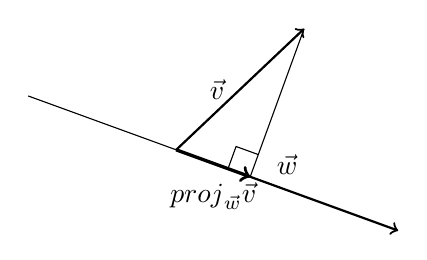
\begin{tikzpicture}[rotate=-20]
\draw [->,thick] (0,0) -- node [left=2pt]{$\vec v$}(1,2);
\draw [->,thick] (0,0) -- node [above=2pt]{$\vec w$}(3,0);
\draw [thin] (-2,0) -- (.7,0) -- (.7,.3) -- (1,.3);
\draw  (1,0) -- (1,2);
\draw [->,very thick] (0,0) -- node[below=3pt]{$\text{proj}_{\vec w}\vec v$} (1,0);
\end{tikzpicture}
\quad
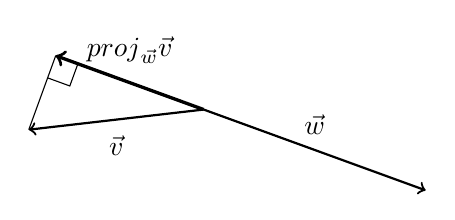
\begin{tikzpicture}[rotate=-20]
\draw [->,thick] (0,0) -- node [below=2pt]{$\vec v$}(-2,-1);
\draw [->,thick] (0,0) -- node [above=2pt]{$\vec w$}(3,0);
\draw [thin] (-2,0) -- (-1.7,0) -- (-1.7,-.3) -- (-2,-.3);
\draw  (-2,0) -- (-2,-1);
\draw [->,very thick] (0,0) -- node[above=3pt]{$\text{proj}_{\vec w}\vec v$} (-2,0);
\end{tikzpicture}
\end{center}
	
	
	
We'll develop a formula for the projection first by using trigonometry, and then second by using facts about inner products and null spaces.  
We start with trigonometry.  
The length of the projection is 
$$\ds|\vec v| \cos \theta = |\vec v|\frac{\vec v\cdot \vec w}{|\vec v||\vec w|} = \frac{\vec v\cdot \vec w}{|\vec w|}.$$ 
A unit vector for the direction of the projection is $\ds\frac{\vec w}{|\vec w|}$. 
Hence we have $$\ds\text{proj}_{\vec w}\vec v = (\text{mag})(\text{dir}) = \left(\frac{\vec v\cdot \vec w}{|\vec w|}\right)\frac{\vec w}{|\vec w|} = \left(\frac{\vec v\cdot \vec w}{\vec w\cdot \vec w}\right)\vec w .$$

In terms of inner products, the projection of $\vec v$ onto $\vec w$ is a vector $c\vec w$ in the direction of $\vec w$ which is ``closest'' to $\vec v$. To be ``closest''means we want the distance from the tip of $\vec v$ to the line containing $\vec w$ to be as small as possible. This occurs precisely when the difference $\vec v-c\vec w$ has the smallest length, which means that $\vec v-c\vec w$ meets $\vec w$ at a 90 degree angle. We need to pick a value $c$ so that $\vec v-c\vec w$ and $\vec w$ are orthogonal, or have an inner product of zero.  Since these two vectors are orthogonal, we need to find $c$ so that 
$$\left<\vec v-c\vec w,\vec w\right>=0.$$
Since the inner product preserves vector addition and scalar multiplication, we seek $c$ so that
$$\left<\vec v,\vec w\right>-c\left<\vec w,\vec w\right>=0$$
Solving for $c$ gives $$ c= \frac{\left<\vec w,\vec w\right>}{\left<\vec v,\vec w\right>}\quad \text{and so the projection is}\quad 
\text{proj}_{\vec w}\vec v = c\vec w=\frac{\left<\vec v,\vec w\right>}{\left<\vec w,\vec w\right>}\vec w.
$$ 
The scalar $c=\frac{\left<\vec v,\vec w\right>}{\left<\vec w,\vec w\right>}$ is called the Fourier coefficient of $\vec v$ with respect to $\vec w$, or the component of $\vec v$ along $\vec w$.

\begin{example}
The projection of $\vec v = (0,3,4)$ onto $\vec w = (2,1,-2)$ is 
$$\ds \text{proj}_{(2,1,-2)}(0,3,4) =\frac{\left<(0,3,4),(2,1,-2)\right>}{\left<(2,1,-2),(2,1,-2)\right>}(2,1,-2) = \frac{-5}{9}(2,1,-2).$$ The number $-5/9$ is the Fourier coefficient of $(0,3,4)$ with respect to $(2,1,-2)$.

The projection of $\vec w = (2,1,-2)$  onto $\vec v = (0,3,4)$ is 
$$\ds \text{proj}_{(0,3,4)}(2,1,-2) =\frac{\left<(2,1,-2),(0,3,4)\right>}{\left<(0,3,4),(0,3,4)\right>}(0,3,4) = \frac{-5}{25}(0,3,4).$$ The number $-5/25 = -1/5$ is the Fourier coefficient of $(2,1,-2)$ with respect to $(0,3,4)$.
 
\end{example}



\subsection{Projecting a vector onto a subspace}

When projecting a vector $\vec v$ onto a vector $\vec w$, we need to find a vector $\text{proj}_{\vec w}\vec v = c\vec w$ in the space spanned by $\vec w$ so that the difference $\vec n = \vec b - c\vec w$ is orthogonal to $\vec w$.  We wanted to make $\vec n  = \vec b-c\vec w$ become a vector in the orthogonal complement of $\vec w$ by carefully choosing $c$. The projection is then simply $\vec b - \vec n$. Before generalizing this process to larger subspaces, let's follow through this process with a specific example to see how the computations work. We will then repeat this process where we replace $\vec w$ with any vector subspace $W$ and learn how to project vectors onto vector subspaces.

\begin{example}
Let's redo the projection example where we project $\vec v = (0,3,4)$ onto $\vec w = (2,1,-2)$.  We want a scalar $c$ so that the vector $\vec v-c\vec w = \bm{0\\3\\4}-c\bm{2\\1\\-2}$ is in the null space of $A^T = \bm{2\\1\\-2}^T = \bm{2&1&-2}$. This means that $A^T (\vec v-c\vec w )=0$ or $A^T c\vec w = A^T \vec v$. With the numbers from this problem, we need to satisfy the matrix equation 
$$\bm{2&1&-2}c\bm{2\\1\\-2} = \bm{2&1&-2}\bm{0\\3\\4} \quad \text {or}\quad c\vec w^T\vec w = \vec w^T\vec v.$$
This is precisely $c (9) = -5$ so $c=-5/9$.  Notice that we obtained $c = \vec w\cdot \vec v/\vec w\cdot \vec w$.
\end{example}

We are now ready to project an arbitrary vector $\vec b$ onto a subspace $W$.  We're using $\vec b$ so that the formula we obtain in the end is precisely the forumla we used to perform linear regression. 
The projection of a vector $\vec b$ onto a subspace $W$ is the vector $\vec w$ in that space whose head is nearest to the head of $\vec b$. 
To find this vector, we seek a vector $\vec n$ in the orthogonal complement of $W$ such that $$\vec b-\vec n=\vec w$$ is a vector in $W$. 
To achieve this, let $A$ be a matrix whose columns form a basis for the space $W$.  
The orthogonal complement of $W$ is the null space of $A^T$.  
So the solutions to $A^T\vec n=\vec 0$ are precisely the vectors in the orthogonal complement of $W$. 
Because the projection $\vec w=\vec b-\vec n$ by definition is in the vector space space $W$, we know that a linear combination of the columns of $A$ will provide this vector $\vec w$.   
Let $\vec x$ be the coordinates of $\vec w$ relative to the basis vectors in $A$, so that 
$$A\vec x = \vec w.$$ 
Multiplying both sides by $A^T$ gives us $$A^T A \vec x = A^T\vec w =A^T\vec b - A^T\vec n = A^T\vec b - \vec 0.$$ 
The vectors $\vec x$ and $\vec b$ satisfy the equation $A^T A \vec x = A^T \vec b$. We can solve this equation for $\vec x$ by inverting the square matrix $A^TA$ to obtain $$\vec x = (A^TA)^{-1} A^T\vec b.$$
We can then find the projection of $\vec b$ onto $W$ as
$$\text{proj}_W\vec b = A\vec x = A (A^TA)^{-1} A^T\vec b.$$

Does this look familiar? Does it look like our linear regression formula? Linear regression is just projecting a vector onto a subspace, where the coefficients of the line are coordinates $\vec x$ of the vector $\vec w$ in the space $W$ that is nearest to $\vec b$. If $S$ is the columns of $A$, then the solution to the least square regression problem is simply $\vec x = [\vec w]_S$ where $\vec w = \text{proj}_A\vec b$.


\begin{example}
Let's find a line that is closest to passing through the three points $(0,1),(2,3),(4,6)$. Suppose for a moment that there were a line of the form $y=mx+b$ that did pass through the points.  Plugging our 3 points into the equation $a_0+a_1x=y$ gives the inconsistent system of equations 
$$\begin{cases}a_0=1\\a_0+2a_1=3\\a_0+4a_1=6\end{cases}
\xrightarrow{\text{augmented matrix}}
\begin{bmatrix}[cc|c]1&0&1\\1&2&3\\1&4&6\end{bmatrix}
\xrightarrow{\text{matrix form}}
\begin{bmatrix}1&0\\1&2\\1&4\end{bmatrix}
\begin{bmatrix}m\\b\end{bmatrix}
=\begin{bmatrix}1\\3\\6\end{bmatrix}.
$$
Notice that the system can be written in matrix form $A\vec x = \vec b$ where $A$ contains a column of 1's and $x$ values, and $\vec b$ is a column of $y$ values.  Because the system above has no solution, we want to find the vector $\vec w = \vec b-\vec n$ in the column space of $A$ (meaning $\vec w=A\vec x$ )where $\vec w$ is the projection of $\vec b$ onto the 2D space spanned by the columns of $A$. In other words, find the shortest vector $\vec n$ such that $\vec w= \vec b-\vec n$ is a solution to $A\vec x = \vec b-\vec n$. The vector $\vec n$ must exist, so multiply both sides by $A^T$ to obtain
$$A^T A \vec x = A^T(\vec b-\vec n) =A^T\vec b - A^T\vec n = A^T\vec b,$$
where $A^T\vec n = \vec 0$ because it is in the orthogonal complement of the columns of $A$ (the shortest vector from $\vec b$ to the column space of $\vec A$ must be orthogonal to the columns of $A$). 
The resulting system has only 2 rows and a symmetric coefficient matrix $A^TA$:
$$A = \begin{bmatrix}1&0\\1&2\\1&4\end{bmatrix}, 
A^T = \begin{bmatrix}1&1&1\\0&2&4\end{bmatrix}, 
A^T A = \begin{bmatrix}3&6\\6&20\end{bmatrix}, 
A^T\vec b = \begin{bmatrix}10\\30\end{bmatrix}, \begin{bmatrix}3&6\\6&20\end{bmatrix} \begin{bmatrix}m\\b\end{bmatrix}=\begin{bmatrix}30\\10\end{bmatrix}.$$ 
Reduce $\begin{bmatrix}[cc|c]3&6&10\\6&20&30\end{bmatrix}$ to $\begin{bmatrix}[cc|c]1&0&5/6\\0&1&5/4\end{bmatrix}$, which means the solution is $y=\frac{5}{6}+\frac{5}{4}x.$  Alternatively, invert $A^TA$ to obtain the solution $$\vec x = (A^T A)^{-1}A^T \vec b = \begin{bmatrix}5/6&-1/4\\-1/4&1/8\end{bmatrix}\begin{bmatrix}10\\30\end{bmatrix} = \begin{bmatrix}5/6\\5/4\end{bmatrix}.$$  

\end{example} 

Let's revisit the previous example but this time use the language of projections and orthogonal complements.

\begin{example}
Let's find the projection of $\vec b = (1,3,6)$ onto the space $$W=\text{span}\{(1,1,1),(0,2,4)\}.$$ If $\vec w =\text{proj}_{W}\vec b$, then $\vec n=\vec b-\vec w$ is in the null space of the transpose of $A = \begin{bmatrix}1&0\\1&2\\1&4\end{bmatrix}$, so $A^T(\vec b - \vec w)=\vec 0$, or $A^T\vec w =A^T\vec b$.  Since $\vec w$ is in the column space of $A$, we know that $\vec w = A\vec x$ for some $x$.  We now solve $A^T A \vec x = A^T\vec b$. The computations are the same as the previous example, and we obtain $\vec x = (5/6,5/4)$.  This means 
$$\text{proj}_W\vec b = A\vec x = \begin{bmatrix}1&0\\1&2\\1&4\end{bmatrix}\begin{bmatrix}5/6\\5/4\end{bmatrix} = \begin{bmatrix} 
 {5}/{6} \\
 {10}/{3} \\
 {35}/{6}
\end{bmatrix}.$$
The numbers $(5/6,5/4)$ are the coordinates of the projection relative to the columns of $A$ (a basis for the column space).
\end{example}







\section{Orthogonal and Orthonormal}

The least squares regression problem introduced an idea related to finding the projection of a vector $\vec b$ onto a vector subspace $W$.  This requires that we obtain a basis for the space $W$. Once we have picked a basis, then the projection $A\vec x=\vec w$ must satisfy $A^TA\vec x = A^T\vec b$, where $\vec x$ is the coordinates of $\vec w$ relative to our basis. Solving for $\vec x$ we obtain $\vec x = (A^T A)^{-1}A^T \vec b$. To find the projection $\vec w = A\vec x$, we multiply by $A$ to obtain $$\vec w = \text{proj}_W \vec b =  A\vec x = A(A^T A)^{-1}A^T \vec b.$$ The coordinates of $\vec w$ relative to this basis are $\vec x = (A^T A)^{-1}A^T \vec b$, and are called the Fourier coefficients of $\vec b$ relative to the basis chosen for $W$.
In the next section we will show how to obtain a ``nice'' basis so that obtaining the projection and its coordinates is very simple. As always, this requires that we pick a good basis in which to perform computations.


The standard basis vectors $(1,0,0),(0,1,0),(0,0,1)$ are each orthogonal to the other, so we say they are an \textbf{orthogonal set of vectors}.
\marginpar{An orthogonal set of vectors is a set where each vector is orthogonal to all the others.}
These standard basis vectors are also all unit vectors; they all have norm 1. 
Because they are all unit vectors and orthogonal, we say they form an \textbf{orthonormal} set of vectors. 
\marginpar{An orthonormal set of vectors is an orthogonal set where each vector has norm 1.}
As we proceed throughout this section, we will find that when you choose as your basis an orthonormal set of vectors, computations related to projections and inversion become extremely simple (hence computer programmers prefer to work with orthonormal bases). 
The telecommunications industry works with an orthonormal basis because computations are extremely fast with this basis.

\begin{example}
The set of vectors $(2,-1,0), (1,2,0),(0,0,1)$ forms an orthogonal set because the dot product of any two vectors is zero (check this).  
Normalizing each vector (dividing by its magnitude) gives the set $(\frac{2}{\sqrt5},-\frac{1}{\sqrt5},0), (\frac{1}{\sqrt5},\frac{2}{\sqrt5},0),(0,0,1)$, which is an orthonormal set of vectors. 
\end{example}

Let $A = \bm{\vec w_1&\vec w_2&\cdots&\vec w_n}$ be a matrix whose columns form an orthogonal set of vectors. Because the vectors are orthogonal, if $i\neq j$ then $\vec w_i\cdot\vec w_j=0$. To compute the matrix product $A^T A$, we take row $i$ of $A^T$ and dot it with column $j$.  But row $i$ of $A^T$ is the same as column $i$ of $A$, so the $ij$ entry in $A^TA$ is zero if $i\neq i$.  This means that $A^TA$ is a diagonal matrix. The diagonal entries are simply $\vec w_i\cdot \vec w_i = |\vec w_i|^2$, the square of the length of the vectors. Diagonal matrices are extremely simple to work with and invert.

In terms of projections, if we choose basis vectors $S =\{ \vec w_1,\ldots,  \vec w_n\}$ for $W$ that are orthogonal, then $A^T A$ is a diagonal matrix (the diagonal entries are the square of the lengths of the basis vectors), and the coordinates of our projection relative to this basis (the Fourier coefficients) are (inverting a diagonal matrix is just inverting each diagonal entry)
\begin{align*}
\vec x = (A^T A)^{-1}A^T \vec b 
&=\left(\bm{\vec w_1^T\\\vec w_2^T\\\vdots\\\vec w_n^T}\bm{\vec w_1&\vec w_2&\cdots&\vec w_n}\right)^{-1} \bm{\vec w_1^T\\\vec w_2^T\\\vdots\\\vec w_n^T}\vec b\\
&=\bm{\vec w_1^T\vec w_1&0&\cdots&0\\0&\vec w_2^T\vec w_2&\ddots&0\\\vdots&\ddots&\ddots&\vdots\\\vec w_n^T\vec w_n}^{-1} \bm{\vec w_1^T\vec b\\\vec w_2^T\vec b\\\vdots\\\vec w_n^T\vec b}\\
&=\bm{\frac{1}{\left<\vec w_1,\vec w_1\right>}&0&\cdots&0\\0&\frac{1}{\left<\vec w_2,\vec w_2\right>}&\ddots&0\\\vdots&\ddots&\ddots&\vdots\\0&0&\cdots&\frac{1}{\left<\vec w_n,\vec w_n\right>}}^{-1} \bm{\left<\vec w_1,\vec b\right>\\\left<\vec w_2,\vec b\right>\\\vdots\\\left<\vec w_n,\vec b\right>} 
= 
\bm{ \frac{\left<\vec w_1,\vec b\right>}{\left<\vec w_1,\vec w_1\right>} \\ \frac{\left<\vec w_2,\vec b\right>}{\left<\vec w_2,\vec w_2\right>}  \\ \vdots \\  \frac{\left<\vec w_n,\vec b\right>}{\left<\vec w_n,\vec w_n\right>}  }
.\end{align*}
The coordinates $\vec x = (c_1, \ldots, c_n)$ are found by computing the inner product of each row with $\vec b$ and dividing by the length of that row, or 
$$c_i = \frac{\vec w_i^T\vec b}{\vec w_i^T\vec w_i} = \frac{\vec w_i\cdot \vec b}{\vec w_i\cdot \vec w_i} = \frac{\left<\vec w_i, \vec b\right>}{\left<\vec w_i, \vec w_i\right>}  \quad \quad \text{ (Fourier coefficients)}.$$

If we choose basis vectors $S$ that are orthonormal (so $\left<\vec w_i,\vec w_i\right>=1$), then $A^TA$ is simply the identity matrix. This means $\vec x = (A^TA)^{-1}A^T \vec b = A^T\vec b$ and so the projection of $\vec b$ onto $W$ is $\vec w = AIA^T\vec b$.  The coordinates of $\vec w$ relative to this basis (called Fourier coefficients) are simply $\vec x = A^T \vec b$. Notice that this means the coordinates $\vec x = (c_1, \ldots, c_n)$ are found by computing the inner product of each row with $\vec b$ (no division is needed because each vector has length 1). Using symbols, if $\{\vec w_1,\ldots, \vec w_n\}$ is an orthonormal basis for $W$, then the Fourier coefficients of $\vec b$ relative to this basis are $$c_i = \vec w_i^T\vec b = \vec w_i\cdot \vec b = \left<\vec w_i,\vec b_i\right>.$$
Everything we have developed works in any vector space provide you have an inner product.

\begin{example}
What is the projection of $(3,-2,5)$ onto the space spanned by the vectors $\vec v_1=(2,-1,0)$ and $\vec v_2 = (1,2,0)$? 
Since the vectors are orthogonal (check that their dot product is 0), we can find the Fourier coefficients by dotting each $\vec v_i$ with $\vec b$ and dividing by the square of the length.  We obtain 
$$c_1 =  \frac{\left<\vec v_1, \vec b\right>}{\left<\vec v_1, \vec v_1\right>}
= \frac{\left<(2,-1,0), (3,-2,5)\right>}{\left<(2,-1,0), (2,-1,0)\right>} =  \frac{8}{5},$$
$$ c_2 =  \frac{\left<\vec v_2, \vec b\right>}{\left<\vec v_2, \vec v_2\right>}
= \frac{\left<(1,2,0), (3,-2,5)\right>}{\left<(1,2,0), (1,2,0)\right>} =  \frac{-1}{5}.$$
This means the projection is $$\vec w = c_1\vec v_1+c_2\vec v_2 = \frac{8}{5}(2,-1,0) + \frac{-1}{5}(1,2,0) = \frac{(16-1,-8-2,0)}{5} = (3,-2,0).$$

Let's consider the same set of vector, but now use an orthonormal basis to do the projection. These vectors are orthogonal, so normalizing them (divide by their magnitude) yields the orthonormal set of vectors $\vec w_1 = \frac{1}{\sqrt{5}}(2,-1,0), \vec w_2=\frac{1}{\sqrt{5}}(1,2,0)$.  The coefficients of the projection (the Fourier coefficients relative to the orthonormal basis) are hence 
$$c_1 = \vec w_1\cdot \vec b = \frac{1}{\sqrt{5}}(2,-1,0)\cdot (3,-2,5) = \frac{8}{\sqrt{5}}, \quad c_2 =  \vec w_2\cdot \vec b = \frac{1}{\sqrt{5}}(1,2,0)\cdot (3,-2,5) = \frac{-1}{\sqrt{5}}.$$ This means the projection $\vec w$ onto the space is 
\begin{align*}
\vec w = c_1 \vec w_1 + c_2\vec w_2 
= \frac{8}{\sqrt{5}} \vec w_1 + \frac{1-}{\sqrt{5}}\vec w_2 
&= \frac{8}{\sqrt{5}} \frac{1}{\sqrt{5}}(2,-1,0) + \frac{-1}{\sqrt{5}}\frac{1}{\sqrt{5}}(1,2,0) \\
&= \frac{1}{5}(16-1,-8-2,0) = (3,-2,0).
\end{align*}
\end{example}

Computer programs prefer to work with orthonormal bases because with them you can avoid the division by the square of the length of each basis vectors.  When working with problems by hand, we'll often just use an orthogonal basis that avoids fractions.  This way we can focus on the ideas at hand and then at the very end include the division.

\subsection{Gram-Schmidt Orthogonalization Process}


Given a set of linearly independent vectors $\{\vec v_1,\ldots,\vec v_n\}$, how do I create a set of orthonormal vectors $\{\vec w_1,\ldots,\vec w_n\}$ whose span is the same as the span of the original vectors?  Start with your first vector and let $\vec w_1 = \vec v_1$.  Since $\vec v_2$ is not in the space spanned by $\vec w_1$, find the projection of $\vec v_2$ onto $\vec w_1$ and then let $\vec w_2$ be $\vec v_2$ minus this projection, $w_2 = v_2 - \frac{\left<\vec v_2,\vec w_1\right>}{\left<\vec w_1,\vec w_1\right>}\vec w_1.$ This means that $\vec w_1$ and $\vec w_2$ are orthogonal, and they span the same space as $\vec v_1$ and $\vec v_2$.  Since $\vec v_3$ is not in the space spanned by $\vec w_1$ and $\vec w_2$, find the projection of $\vec v_3$ onto the plane spanned by $\vec w_1$ and $\vec w_2$ and then let $\vec w_3$ be $\vec v_3$ minus this projection, 
$w_3 = v_3 
- \frac{\left<\vec v_3,\vec w_1\right>}{\left<\vec w_1,\vec w_1\right>}\vec w_1
- \frac{\left<\vec v_3,\vec w_2\right>}{\left<\vec w_2,\vec w_2\right>}\vec w_2.$ This means that $\vec w_1, \vec w_2,$ and $\vec w_3$ are orthogonal, and span the same space as $\vec v_1, \vec v_2, \vec v_3$.  Repeat this process, each time projecting $\vec v_k$ onto the subspace generated by the $k-1$ previous orthogonal vectors.  Once you are done, you will have an orthogonal set of vectors.  Divide each vector by its magnitude to obtain an orthonormal set.  Schaum's has a description of this on page 255.

%add a picture when you have time

\begin{example}
Example 7.13 in the book (page 256) illustrates this nicely. Due to time constraints, I won't have my own example here.
\end{example}


\subsection{Orthogonal Matrices}
We have seen in chapter 5 that many problems become simpler when we can find a basis that diagonalizes a linear transformation. If $P$ is a similarity matrix that diagonalizes $A$, then $D=P^{-1}AP$ is the diagonal matrix.  As matrices become larger, finding the inverse or $P$ is perhaps the most time intensive part of this computation.  This section shows that when $A$ is a symmetric matrix, it is always possible to find a basis such that the inverse of $P$ is extremly simple, namely $P^{-1} = P^T$ (the inverse is the transpose). To introduce this idea, let's start with a simple example.

\begin{example}
The matrix $A = \bm {2&1\\1&2}$ has eigenvalues $3,1$ with eigenvector $(1,1)$ and $(-1,1)$. 
Notice that these two eigenvectors are orthogonal as $(1,1)\cdot(-1,1)=0$. 
If we let $P = \bm{1&-1\\1&1}$, then $\ds P^{-1} = \frac{1}{2}\bm{1&1\\-1&1} = \frac{1}{2}P^T$, almost the transpose.
The vectors we choose were orthogonal, but not normalized. Since eigenvectors can be multiplied by any scalar and still remain as eigenvectors, let's use the vectors $\frac{1}{\sqrt{2}}(1,1)$ and $\frac{1}{\sqrt{2}}(-1,1)$ instead. With these eigenvectors, we have 
$$P = \bm{1\sqrt{2}&-1\sqrt{2}\\1\sqrt{2}&1\sqrt{2}}, \quad P^{-1} = \bm{1\sqrt{2}&1\sqrt{2}\\-1\sqrt{2}&1\sqrt{2}} = P^T,\quad
\text{and}\quad D = \bm{3&0\\0&1} = P^T A P.$$ 
The inverse of $P$ is extremely simple and we can replace $D=P^{-1}AP$ with $D=P^T A P$.  
\end{example}

Now it's time for some language.
\begin{definition}
A matrix is said to be orthogonal if $A^TA=AA^T=I$, or in other words $A^T=A^{-1}$ (the transpose is the inverse).  
\end{definition}
\marginpar{Schaum's has more examples on pages 113-114.} If $\vec u_i$ is the $i$th column of $A$, then the product $A^TA$ has in  the $ij$th spot the product $\vec u_i^T \vec u_j$.  In order for a matrix to be orthogonal, this requires that $\vec u_i^T \vec u_j=0$ if $i\neq j$ (so columns $i$ and $j$ are orthogonal) and that $\vec u_i^T \vec u_j=1$ when $i=j$ (so each vector has length 1).  We have just proved the following theorem
\begin{theorem}
The following three conditions are equivalent for a square matrix $A$:
\begin{enumerate}
	\item $A$ is orthogonal - meaning $A^TA=AA^T=I$.
	\item The columns of $A$ form an orthonormal set.
	\item The rows of $A$ form an orthonormal set.
\end{enumerate}
\end{theorem}
The key use we'll make of this theorem is that if a similarity matrix $P$ has orthonormal columns, then its inverse is the transpose, and we can diagonalize $A$ by writing $D=P^TAP$. 

\begin{example}
See example 7.14 in Schaum's (page 257). Part b is a rotation matrix. Every rotation in any dimension is represented by an orthogonal matrix, so computer graphic designers use these all the time.
\end{example}


\subsection{Diagonalizing Symmetric Matrices}

If $A$ is a matrix that can be diagonalized by an orthogonal matrix, then what can be said about $A$?  We'll show that $A$ must be symmetric ($A^T=A$).  Here's why.  If $D = P^T A P$, then multiply on the left by $P$ and on the right by $P^T=P^{-1}$ to obtain $A=P DP^T$. The transpose of $A$ is hence (reverse the order and transpose each) 
$$A^T = (PDP^T)^T = P^T D^T (P^T)^T = P^T D P^T = A,$$ since $D^T=D$ (as a diagonal matrix) and $(P^T)^T=P$.
Hence, the only kinds of matrices that can be diagonalized with an orthogonal matrix are precisely symmetric matrices.

Symmetric matrices appeared earlier in the semester when we studied optimization and the second derivative test.  They also appeared at the beginning of the unit as every inner product can be represented by a symmetric matrix.  Much has been learned about symmetric matrices. We now state a key theorem about symmetric matrices.
\begin{theorem}[Real Spectral Theorem]
Let $A$ be a symmetric matrix. 
\begin{enumerate}
	\item All the eigenvalues of $A$ are real.
	\item For each eigenvalue, the geometric multiplicity matches the algebraic multiplicity.
	\item Eigenvectors corresponding to different eigenvalues are orthogonal.
\end{enumerate}
In particular, these three facts imply that every symmetric matrix can be diagonalized by an orthogonal matrix of real numbers (the Gram-Schmidt process may have to be used if an eigenvalue occurs with algebraic multiplicity more than one). 
\end{theorem}

\begin{example}
See page 404 in Schaum's, example 11.9.  
When finding the characteristic polynomial, you can either compute the trace and determinant to find the coefficients, or you can subtract $\lambda$ from the diagonals and then find the determinant. 
\end{example}

Now, do you remember the second derivative test we learned at the beginning of the semester?  Every matrix involved in the second derivative test will always be symmetric.  This means that with every 2nd derivative test (optimization problem), you will always be able to find the eigenvalues and they will be real numbers.  
In addition, a basis of eigenvectors can be chosen to always meet at right angles. 
Changing bases is a way of rearranging how we view a problem, and symmetric matrices have extremely nice bases. 








